\subsection{Case Study: Interconnect Messaging}

\begin{figure}[!htbp]

\begin{center}
\begin{subfigure}[b]{\linewidth}
  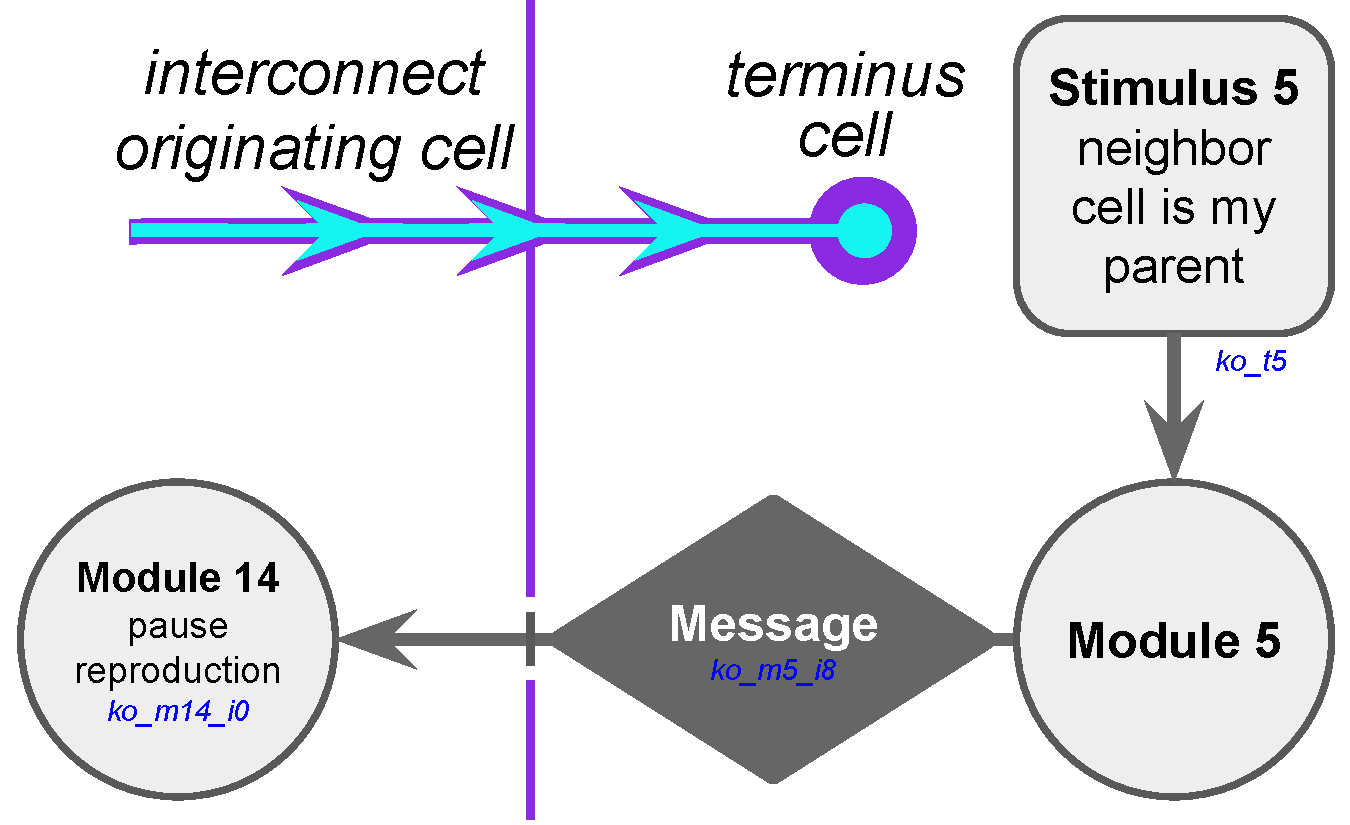
\includegraphics[width=\linewidth,clip]{batch=2032+step=1018+pop=0/2032_diagram}
  \caption{Hypothesized selective reproduction pausing mechanism}
  \label{fig:mechanism2}
\end{subfigure}
\begin{subfigure}[b]{0.45\linewidth}
  
\includegraphics[width=\linewidth,trim={0 200 200 0},clip]{batch=2032+step=1018+pop=0/seed=1+title=channel+treat=batch_2032,step_1018,pop_1,id1_wt+update=5000+_emp_hash=0c549f0-clean+_source_hash=d50b431-dirty+ext=}
  \caption{Kin groups}
  \label{fig:kingroups2}
\end{subfigure}
\begin{subfigure}[b]{0.45\linewidth}
  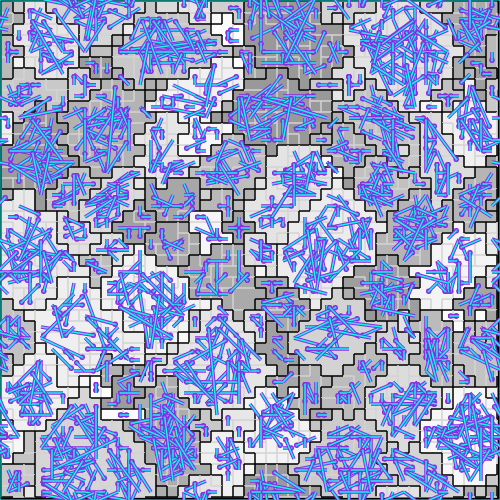
\includegraphics[width=\linewidth,trim={0 200 200 0},clip]{batch=2032+step=1018+pop=0/seed=1+title=established-interconnect+treat=batch_2032,step_1018,pop_1,id1_wt+update=5000+_emp_hash=0c549f0-clean+_source_hash=d50b431-dirty+ext=}
  \caption{Established interconnects}
  \label{fig:establishedinterconnects2}
\end{subfigure}
\begin{subfigure}[b]{0.45\linewidth}
  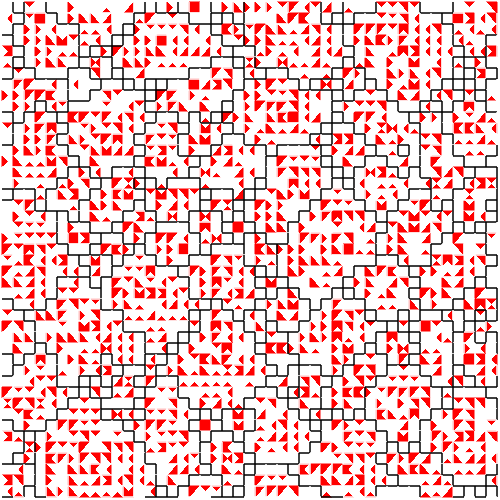
\includegraphics[width=\linewidth,trim={0 200 200 0},clip]{batch=2032+step=1018+pop=0/seed=1+title=parent-cell-of+treat=batch_2032,step_1018,pop_1,id1_wt+update=5000+_emp_hash=0c549f0-clean+_source_hash=d50b431-dirty+ext=}
  \caption{Spatial distriubiton of stimulus 5TODO fix}
  \label{fig:t5distribution}
\end{subfigure}
\begin{subfigure}[b]{0.45\linewidth}
  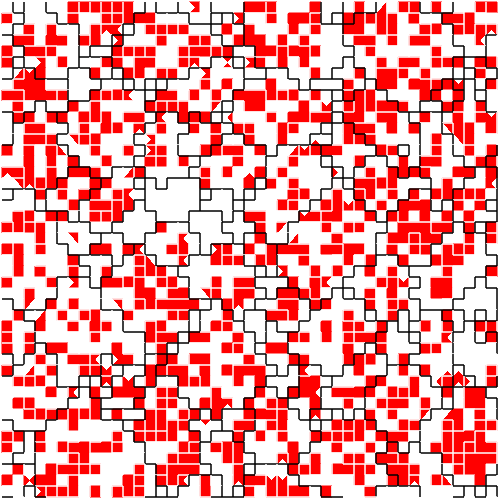
\includegraphics[width=\linewidth,trim={0 200 200 0},clip]{batch=2032+step=1018+pop=0/seed=1+title=reproductive-pause-level-0+treat=batch_2032,step_1018,pop_1,id1_wt+update=5000+_emp_hash=0c549f0-clean+_source_hash=d50b431-dirty+ext=}
  \caption{Spatial distribution of module 14 execution}
  \label{fig:m14distribution}
\end{subfigure}
\caption{
Batch 2032 case study overview.
Figures \ref{fig:kingroups2} through \ref{fig:m14distribution} are generated from a snapshot of a wild-type strain monoculture population.
In these images, each grid tile represents an individual cell.
Cells are organized into kin groups, color-coded by hue in Figure \ref{fig:kingroups2}.
Established interconnects are overlaid in blue on Figure \ref{fig:establishedinterconnects2}.
In Figures \ref{fig:t5distribution} and \ref{fig:m14distribution}, kin groups are outlined in black.
Figure \ref{fig:t5distribution} highlights cells that are sending resource over-interconnect.
Figure \ref{fig:m14distribution} highlights cells that are receiving resource over-interconnect.
You can view an animation of the wild-type monoculutre at \url{https://mmore500.com/hopto/an}.
}
\label{fig:case_study_2032}
\end{center}
\end{figure}


This case study was drawn from epoch 18 of batch 32 from the secondary set of evolutionary runs.
%TODO try to rephrase as an inclusive statement to get two birds with one stone
We set this strain aside for case study after preliminary screening suggested that over-interconnect messaging played an adaptive role and that the intercellular nature the messaging of was necessary to that adaptation.
The evolutionary history preceeding this case study consumed approximately 72 hours of wall-clock time and 576 compute-core hours.
Approximately 2,197,976 simulation updates and 8,884 cellular generations elapsed.
You can view this case study strain in a live in-browser simulation at \url{https://mmore500.com/hopto/7}.
% 100%|██████████████████████████████████████████████████████████████████████████████████████████████████████████████████████████████████████████████████████████| 19/19 [00:00<00:00, 406.39it/s]
% Output saved to title=mastergenerations+_data_hathash_hash=4b3da18cbeb2bc0d+_script_fullcat_hash=5e6b7a64514cbb09+_source_hash=29a51b3-clean+ext=.csv
% level 0
% Generations Elapsed mean 8884.38084673059
% Generations Elapsed std nan
% Generations Elapsed min 8884.38084673059
% Generations Elapsed max 8884.38084673059
% level 1
% Generations Elapsed mean 5674.207208163186
% Generations Elapsed std nan
% Generations Elapsed min 5674.207208163186
% Generations Elapsed max 5674.207208163186
% level 2
% Generations Elapsed mean 1196.6607671890404
% Generations Elapsed std nan
% Generations Elapsed min 1196.6607671890404
% Generations Elapsed max 1196.6607671890404
% EXPIRATION_UPDATE 513408
% EXPIRATION_UPDATE 233216
% EXPIRATION_UPDATE 184096
% EXPIRATION_UPDATE 211488
% EXPIRATION_UPDATE 182368
% EXPIRATION_UPDATE 175840
% EXPIRATION_UPDATE 189952
% EXPIRATION_UPDATE 202496
% EXPIRATION_UPDATE 136992
% EXPIRATION_UPDATE 140576
% EXPIRATION_UPDATE 143712
% EXPIRATION_UPDATE 128512
% EXPIRATION_UPDATE 114048
% EXPIRATION_UPDATE 123136
% EXPIRATION_UPDATE 110176
% EXPIRATION_UPDATE 111296
% EXPIRATION_UPDATE 116832
% EXPIRATION_UPDATE 103264
% EXPIRATION_UPDATE 114208
% EXPIRATION_UPDATE 119136
% EXPIRATION_UPDATE 86560
% EXPIRATION_UPDATE 91104
% EXPIRATION_UPDATE 85984
% EXPIRATION_UPDATE 94688
% EXPIRATION_UPDATE 85856
% EXPIRATION_UPDATE 111200
% EXPIRATION_UPDATE 101536
% EXPIRATION_UPDATE 131456
% EXPIRATION_UPDATE 77440
% EXPIRATION_UPDATE 88352
% EXPIRATION_UPDATE 74944
% EXPIRATION_UPDATE 89280
% EXPIRATION_UPDATE 88512
% EXPIRATION_UPDATE 82240
% EXPIRATION_UPDATE 80576
% EXPIRATION_UPDATE 84192
% EXPIRATION_UPDATE 89344
% EXPIRATION_UPDATE 91104
% EXPIRATION_UPDATE 91456
% EXPIRATION_UPDATE 88384
% EXPIRATION_UPDATE 82656
% EXPIRATION_UPDATE 87296
% EXPIRATION_UPDATE 75200
% EXPIRATION_UPDATE 84992
% EXPIRATION_UPDATE 99328
% EXPIRATION_UPDATE 102176
% EXPIRATION_UPDATE 113568
% EXPIRATION_UPDATE 97760
% EXPIRATION_UPDATE 108864
% EXPIRATION_UPDATE 104736
% EXPIRATION_UPDATE 104416
% EXPIRATION_UPDATE 99872
% EXPIRATION_UPDATE 98880
% EXPIRATION_UPDATE 110176
% EXPIRATION_UPDATE 100224
% EXPIRATION_UPDATE 93440
% EXPIRATION_UPDATE 97888
% EXPIRATION_UPDATE 97952
% EXPIRATION_UPDATE 106880
% EXPIRATION_UPDATE 95776
% EXPIRATION_UPDATE 103424
% EXPIRATION_UPDATE 99584
% EXPIRATION_UPDATE 100576
% EXPIRATION_UPDATE 101216
% EXPIRATION_UPDATE 107904
% EXPIRATION_UPDATE 112608
% EXPIRATION_UPDATE 101408
% EXPIRATION_UPDATE 110976
% EXPIRATION_UPDATE 110560
% EXPIRATION_UPDATE 101472
% EXPIRATION_UPDATE 102336
% EXPIRATION_UPDATE 96864
% EXPIRATION_UPDATE 105472
% EXPIRATION_UPDATE 97664
% EXPIRATION_UPDATE 97280
% EXPIRATION_UPDATE 111520

As before, we began by testing the adaptiveness of the intercellular nature of over-interconnect interaction. %TODO rephrase
We performed a competition experiment between the wild-type strain and a variant where over-interconnect messages were re-routed back to the sender.\footnote{
This was an independent replication of the initial experiment (performed as part of a wider screen) that singled out the case study strain for further analysis.
}
The wild-type strain was present in greater abundance at the end of all 16 competitions (one-tailed binomial test; $p < 0.0001$; 2/16 variant strain extinctions; 52 S.D. 3 cell gens elapsed).
So the adaptiveness of over-interconnect messaging does depend on the intercellular nature of that messaging in this strain.

We proceeded to tease apart the evolved cellular mechanisms this messaging interacts with.
We monitored hardware execution of the wild-type strain in a monoculture population to detect which signals, messages, and fork/call instructions activated each SignalGP module. %shorten because we already said it
% put in common things into case study introduction
Referring to a human-readable printout of the strain's evolved genetic programming, we pieced together the hypothesized mechanism shown in Figure \ref{fig:case_study_2032}.
It appears that neighboring a direct cellular offspring stimulates dispatch of an over-interconnect message that induces the recipient to pause somatic reproduction.

Four-hour competition experiments between wild type and knockout strains allowed us to assess the adaptiveness of each component of this mechanism.
We replaced the instruction responsible for over-interconnect messaging with a no-op instruction and observed a corresponding fitness penalty (16/16 knockout strain extinctions; one-tailed binomial test; $p < 0.0001$; 416 S.D. 58 cell gens elapsed; \url{https://mmore500.com/hopto/aa}).
We also replaced the reproduction-pausing instruction executed in response to over-interconnect messaging with a no-op.
This caused a similar fitness penalty (16/16 knockout strain extinctions; 401 S.D. 29 cell gens elapsed).

To double-check whether messaging specifically over interconnects was key to adaptivity we also competed the wild-type strain against variants with the focal over-interconnect messaging instruction substituted for all other possible module-activating instructions:
\begin{itemize}
  \item call (378 S.D. 42 cell gens elapsed; \url{https://mmore500.com/hopto/ac})
  \item fork (377 S.D. 37 cell gens elapsed; \url{https://mmore500.com/hopto/ad})
  \item internal message send (406 S.D 39 cell gens elapsed; \url{https://mmore500.com/hopto/ae})
  \item internal message send-to-all (422 S.D 30 cell gens elapsed; \url{https://mmore500.com/hopto/af})
  \item external message send (377 S.D. 37 cell gens elapsed; \url{https://mmore500.com/hopto/ag})
  \item external message send-to-all (440 S.D. 32 cell gens elapsed; \url{https://mmore500.com/hopto/ah})
\end{itemize}
In each case the substitution variant strain was driven to extinction across all 16 replicate experiments (one-tailed binomial test; $p < 0.0001$).

%Channel versus interconnect viz

The directionality of messaging over the interconnect, however, does not appear to affect fitness.
We tried substituting the wild-type instruction, which dispatches a message from the terminus of an interconnect to its origin, with an instruction that instead dispatches a message from the origin of an interconnect to its terminus.
In competition against wild-type, the wild type strain was more abundant in only ten of 16 replicate competitions (one-tailed binomial test; $p = 0.2272$; 14/16 coalesced to a single strain; 410 S.D. 50 cell gen; \url{https://mmore500.com/hopto/ai}).

Next we assessed the adaptiveness of the particular spatio-temporal pattern of stimulation induced by incoming over-interconnect  messages.
Does this pattern differ from spatially and temporally random stimulation?
If it does, is the non-uniformity of stimulation adaptive?
To assess these questions, we measured the frequency of module 14 activation in a monoculture wild-type population.
Then, we created a variant strain where outgoing over-interconnect messages from module 5 were disabled and, instead, module 14 activated randomly with probability based on the empirical wild-type activation rate.
\footnote{
Because over-interconnect broadcast messages activate all hardware units of a cell, we selected entire cells randomly and activated module 14 on all hardware units.
}
% between updates 1000 (238940 hits) and 1100 (267392 hits) updates -> 28452 / (12*45*45*4) = 0.292716
In effect, this manipulation decouples reproductive pause from the distribution of over-interconnect message delivery and instead couples it to a comparable uniform random distribution.
Indeed, in competition experiments against the wild-type strain this variant fares poorly (16/16 variant strain extinctions; one-tailed binomial test; $p < 0.0001$; 58 S.D. 2 cell gen), suggesting that the pattern of stimulation induced by over-interconnect messaging is meaningfully non-unform.

Does the adaptively non-uniform pattern of stimulation induced by over-interconnect messages depend on non-uniform dispatch of messages from sending cells?
To assess, this question, we measured the per-cell frequency of module 5 activation in a monoculture wild-type population.
We created a variant strain where outgoing over-interconnect messages from module 5 were disabled.
Instead, the over-interconnect message instruction was randomly executed per-cell with uniform probability based on the empirical wild-type execution rate.
This variant strain held its own against the wild-type strain (TODO).
So, this strain's non-uniform pattern of stimulation seems likely to a result from the actual pattern of cell-cell interconnection rather than selective message dispatch.

We did not find evidence that cells were using tag-based developmental attractors or repulsers to bias connectivity (TODO).
However, we did notice frequent interconnect turnover via execution of both remove-incoming and remove-outgoing interconnect instructions.
Substituting these instructions for no-ops yielded a knockout strain with lower fitness than wild-type (TODO).
Is this remodeling of connectivity adaptively non-uniform?
We measured the interconnect removal rate in a monoculture wild-type population.
Then, we created a variant strain where interconnect-removal instructions were disabled.
Instead, interconnects in this strain were removed randomly with uniform probability.
In head-to-head competitions this variant strain exhibited equivalent fitness to wild type (TODO).


Although the adaptive mechanism remains hazy, this strain appears to somehow be to meaningfully incorporate into

One possible explanation for the adaptiveness of over-interconnect messaging would be as a proxy for cell age.
Older cells are more likely to have an established interconnect through which to receive stimulation of module 14.
So over-interconnect messaging is adaptive insofar as it associates module 14 activation with cell age.
However, no purely-temporal hypotheses seems likely to fully explain the adaptiveness of over-interconnect messaging:
self-messaging, which experienced .
Although, perhaps through the random-walk developmental process, some sort of spatial information about

Under this line of reasoning,
The distribution of on individual cells, too,
The random-walk developmental process.
However,

However, the established
the random-walk process that interconnects cells.
not just cell age: self-connect
% between updates 1000 and 1100, before ttoal 16613 after total 10883
Incorporates information about multicellular-context of a cell
However,
By the random walk , cell age (and the probability of establishing an interconnect)


This suggests that, together, the conjunction of stimulus 5 on a cell and the presence (via a developmental process) of an interconnect to that cell induces a meaningfully (with respect to fitness) non-uniform distribution of message delivery and, subsequently, module 14 activation.
% break this up into more sentences

next we asked TODO
Does the specific distribution of stimulus 5 on message-generating cells contribute to fitness?
As a rough initial exploration of this question, we performed competition experiments with variants where stimulus 5 was always activated, was never activated, and had inverted activation.
In each case, the variant strain was driven to extinction in all 16 replicate runs (one-tailed binomial test; $p < 0.0001$; 48 S.D. 3 cell gens elapsed; 52 S.D. 3 cell gens elapsed; 48 S.D. 3 cell gens elapsed).
Next, we prepared a variant to test if a uniform stimulus distribution with comparable frequency to wild type would exhibit full fitness.
We empirically measured the stimulus 5 activation rate in a monoculture population of the wild-type strain. TODO
%(observe trigger frequency of 22729/(22729+82571) between 1000 and 1100 updates in a monoculture population)
This variant strain also underperformed wild type, being driven to extinction in all 16 replicate competition runs (62 S.D. 3 cell gens elapsed).

Finally, we
It is also possible that the developmental and process contributes other information to the mix
To randomly select (or select from a distribution).

%TODO Figure \ref{fig:case_study_1042}


